% Filename: p3_preamble@latex_with_vim.tex
% This code is part of LaTeX with Vim.
% 
% Description: LaTeX with Vim is free book about Vim, LaTeX and Git.
% 
% Created: 29.03.12 11:44:40 PM
% Last Change: 30.03.12 12:03:46 AM
% 
% Author: Raniere Gaia Costa da Silva, r.gaia.cs@gmail.com
% Organization:  
% 
% Copyright (c) 2010, 2011, 2012, Raniere Gaia Costa da Silva. All rights 
% reserved.
% 
% This file is license under the terms of a Creative Commons Attribution 
% 3.0 Unported License, or (at your option) any later version. More details
% at <http://creativecommons.org/licenses/by/3.0/>.
\chapter{Preâmbulo} \label{sch:latex:preamble}
Neste capítulo abordaremos o \textit{preâmbulo} do arquivo \lcode{.tex} e a formatação da folha do documento a ser gerado.

\section{\textbackslash\lcode{documentclass} e \textbackslash\lcode{usepackage}}

O \textit{preâmbulo} deve ser iniciado por
\begin{latexcode}
    \documentclass[options]{class}
\end{latexcode}
onde \lcode{class} indica o tipo de documento a ser criado e \lcode{options} personaliza o compartamento de \lcode{class}. Os parâmetros para \lcode{options} devem ser separados por vírgula.

O parâmetro para \lcode{class} corresponde ao nome de um arquivo \lcode{.cls}, os principais são apresentados na Tabela \ref{tab:documentclass} e outros são indicados em \url{http://aprendolatex.wordpress.com/2007/07/15/mais-classes-de-documentos/}. Existe ainda alguns arquivos \lcode{.cls} personalizados disponíveis na internet, destacando-se o \lcode{abnt.cls}, disponível em \url{http://abntex.codigolivre.org.br/}, indicado para documentos que devem seguir as normas da ABNT.
\begin{table}[h!tb]
    \centering
    \caption{Parâmetros disponíveis para \lcode{class}.} \label{tab:documentclass}
    % Filename: documentclass@latex_with_vim.tex
% This code is part of LaTeX with Vim.
% 
% Description: LaTeX with Vim is free book about Vim, LaTeX and Git.
% 
% Created: 30.03.12 12:12:55 AM
% Last Change: 30.03.12 12:13:08 AM
% 
% Author: Raniere Gaia Costa da Silva, r.gaia.cs@gmail.com
% Organization:  
% 
% Copyright (c) 2010, 2011, 2012, Raniere Gaia Costa da Silva. All rights 
% reserved.
% 
% This file is license under the terms of a Creative Commons Attribution 
% 3.0 Unported License, or (at your option) any later version. More details
% at <http://creativecommons.org/licenses/by/3.0/>.
\begin{tabular}{lp{0.8\textwidth}}
    \hline
    Código & Descrição \\ \hline
    \lcode{article} & Para artigos em revistas especializadas, palestras, trabalhos de disciplinas \dots \\
    \lcode{report} & Para informes maiores que constam de mais de um capítulo, projetos de fim de curso, dissertações, teses e similares. \\
    \lcode{book} & Para livros. \\
    \lcode{slide} & Para transparências. \\
    \lcode{beamer} & Para apresenta\c{c}\~{o}es. \\
    \lcode{exam} & Para lista de exerc\'{i}cios. \\
    \hline
\end{tabular}

\end{table}

Na Tabela \ref{tab:par_options} encontramos alguns dos parâmetros disponíveis para \lcode{options}.
\begin{table}[h!tb]
    \centering
    \caption{Parâmetros disponíveis para \lcode{options}.}
    \label{tab:par_options}
    \begin{tabular}{llp{0.6\textwidth}}
        \hline
        Função & Código & Descrição \\ \hline
        \multirow{4}{*}{Tamanho} &  & Utiliza, por padrão, o tamanho 10. \\
        & \lcode{10pt} & Tamanho 10. \\
        & \lcode{11pt} & Tamanho 11. \\
        & \lcode{12pt} & Tamanho 12. \\ \hline
        \multirow{7}{*}{Papel} & & Utiliza, por padrão, o tamanho da folha correspondente carta. \\
        & \lcode{letterpaper} & Tamanho da folha correspondente carta. \\
        & \lcode{a4paper} & Tamanho da folha correspondente a A4. \\
        & \lcode{a5paper} & Tamanho da folha correspondente a A5. \\
        & \lcode{b5paper} & Tamanho da folha correspondente a B5. \\
        & \lcode{executivepaper} & Tamanho da folha correspondente a folha executiva. \\
        & \lcode{legalpaper} & Tamanho da folha correspondente a folha legal. \\ \hline
        \multirow{2}{*}{Al. equação} & & Por padrão centra as equações. \\
        & \lcode{fleqn} & Alinha as equações à esquerda. \\ \hline
        \multirow{2}{*}{Nº equação} & & Por padrão enumera as equações à direita. \\
        & \lcode{leqno} & Enumera as equações à esquerda. \\ \hline
        \multirow{4}{*}{Título} & & Por padrão a classe \lcode{article} não começa uma nova página após o título, enquanto que \lcode{report} e \lcode{book} o fazem. \\
        & \lcode{titlepage} & Começa uma nova página após o título. \\
        & \lcode{leqno} & Não começa uma nova página após o título. \\ \hline
        \multirow{4}{*}{Faces} & & Por padrão a classe \lcode{article} e \lcode{report} são a uma face e a classe \lcode{book} é a duas. \\
        & \lcode{oneside} & Gera o documento a uma face. \\
        & \lcode{twoside} & Gera o documento a duas fazes. \\ \hline
        \multirow{5}{*}{Começo} & & Não funciona com a classe \lcode{article} por nesta não existirem capítulos e por padrão a classe \lcode{report} começa os capítulos na próxima página disponível e a classe \lcode{book} sempre nas páginas à direita. \\
        & \lcode{openright} & Começa os capítulos sempre nas páginas à direita. \\
        & \lcode{openany} & Começa os capítulos na próxima página disponível. \\ \hline
        Colunas & \lcode{twocolumn} & Gera o arquivo utilizando-se de duas colunas. \\
        \hline
    \end{tabular}
\end{table}

O \textit{preâmbulo} do arquivo \lcode{.tex} é completado com os comandos para ativação dos pacotes que adicionam melhorias ao LaTeX que serão utilizados na \textit{informação}. O comando para ativação dos pacotes segue a seguinte sintaxes:
\begin{latexcode}
    \usepackage[options]{package}
\end{latexcode}
onde \lcode{package} é o nome do pacote a ser ativado e \lcode{options} é uma lista de palavras chaves que ativam funções especiais do pacote.

Neste ponto, vale destacar que as distribuições MikTeX e TeX Live possuem os pacotes de uso mais frequentes, mas algumas vezes pode ser necessário baixar o pacote requisitado. No CTAN (The Comprehensive TeX Archive Network: \url{http://www.ctan.org/}) é possível encontrar vários pacotes e a documentação dos mesmos.\footnote{Ao longo do livro, quando for necessário o uso de algum pacote faremos a indicação do mesmo.}

\section{Margens e estilo}

Para cada opção de papel definido em \textbackslash\lcode{documentclass} existe valores padrões para as margens. A seguir, mostraremos algumas maneiras de modificar tais valores e em seguida abordaremos os estilos das páginas.

\subsection{\textbackslash\lcode{setlength} e \textbackslash\lcode{addtolength}}

O comando
\begin{latexcode}
    \setlength{parameter}{length}
\end{latexcode}
atribui o valor \lcode{length} a \lcode{parameter} enquanto que o comando
\begin{latexcode}
    \addtolength{parameter}{length}
\end{latexcode}
adiciona o valor \lcode{length} ao valor padrão correspondente ao \lcode{parameter}.

Para \lcode{length} pode-se utilizar qualquer unidade suportada pelo LaTeX e os \lcode{parameter} disponíveis são apresentados na Tabela \ref{tab:par_margem} e ilustrados na Figura \ref{fig:par_margem}.
\begin{table}[h!tb]
    \centering
    \caption{Opções disponíveis para \lcode{parameter}.}
    \label{tab:par_margem}
    \begin{tabular}{lp{0.8\textwidth}}
        \hline
        Código & Descrição \\ \hline
        \textbackslash\lcode{hotset} & Valor a ser adicionado a margem lateral padrão de uma polegada. \\
        \textbackslash\lcode{votset} & Valor a ser adicionado a margem superior padrão de uma polegada. \\
        \textbackslash\lcode{evensidemargin} & Distância entre a margem lateral e a caixa de texto. \\
        \textbackslash\lcode{topsidemargin} & Distância entre a margem superior e o cabeçalho. \\
        \textbackslash\lcode{headheight} & Altura do cabeçalho. \\
        \textbackslash\lcode{headsep} & Distância entre o cabeçalho e a caixa de texto. \\
        \textbackslash\lcode{textheight} & Altura da caixa de texto. \\
        \textbackslash\lcode{textwidth} & Largura da caixa de texto. \\
        \textbackslash\lcode{marginparsep} & Distância entre a caixa de texto e as notas laterais \\
        \textbackslash\lcode{marginparwidth} & Largura das notas laterais \\
        \textbackslash\lcode{footskip} & Limite inferior para notas de rodapé. \\ \hline
    \end{tabular}
\end{table}
\begin{figure}[h!]
    \centering
    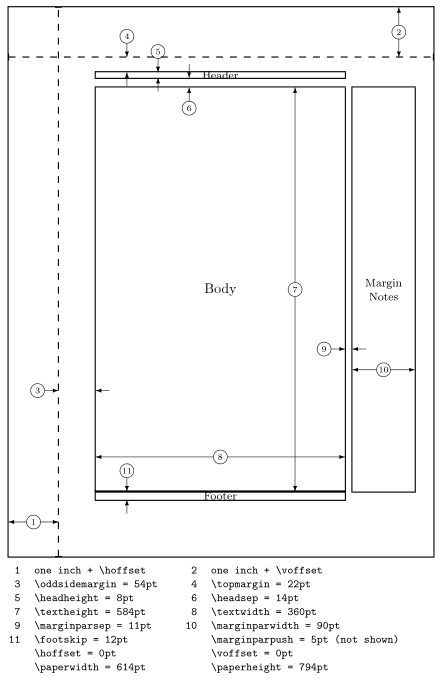
\includegraphics[height=15cm]{figures/margin.png}
    \flushright Fonte: \cite{Graetzer:2007:MoreMath}
    \caption{Ilustração da opções disponíveis para \lcode{parameter} apresentadas na Tabela \ref{tab:par_margem}.} \label{fig:par_margem}
\end{figure}

\subsection{\lcode{geometry}}

Outra maneira de configurar as margens é utilizando o pacote \lcode{geometry}. O uso deste pacote é bastante simples, precisa-se apenas fazer a chamada do pacote e atribuir valores para os parâmetros disponíveis. A seguir apresentamos um exemplo:
\begin{latexcode}
    \usepackage{geometry}
    \geometry{parameter = length, ...}
\end{latexcode}

Assim como para \textbackslash\lcode{setlength} e \textbackslash\lcode{addtolength} podemos utilizar \lcode{length} em qualquer unidade disponível no LaTeX. Já as opções para \lcode{parameter} mais utilizadas são apresentadas na Tabela \ref{tab:par_geometry} e ilustradas na Figura \ref{fig:par_geometry}.
\begin{table}[h!tb]
    \centering
    \caption{Opções disponíveis para \lcode{parameter}, referente ao pacote \lcode{geometry}.}
    \label{tab:par_geometry}
    \begin{tabular}{lp{0.8\textwidth}}
        \hline
        Código & Descrição \\ \hline
        \lcode{paperwidth} & Largura do papel. \\
        \lcode{paperheight} & Altura do papel. \\
        \lcode{textwidth} & Largura da caixa de texto. \\
        \lcode{textheigth} & Altura da caixa de texto. \\
        \lcode{top} & Margem superior. \\
        \lcode{bottom} & Margem inferior. \\
        \lcode{lefth} & Margem esquerda. \\
        \lcode{right} & Margem direita. \\ \hline
    \end{tabular}
\end{table}
\begin{figure}[h!]
    \centering
    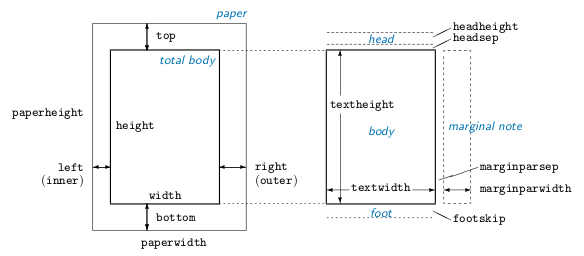
\includegraphics[width=0.8\textwidth]{figures/geometry_margin.png}
    \flushright Fonte: \cite{Moses:2007:Listings}
    \caption{Ilustração da opções disponíveis para \lcode{parameter} apresentadas na Tabela \ref{tab:par_geometry}.} \label{fig:par_geometry}
\end{figure}

\subsection{\textbackslash\lcode{pagestyle}}

Existe um estilo de página definido como padrão\footnote{Corresponde ao estilo \lcode{plain} apresentado na Tabela \ref{tab:par_style}.}, quando deseja-se mudar o estilo em todo o documento pode-se utilizar o comando
\begin{latexcode}
    \pagestyle{style}
\end{latexcode}
e quando for necessário mudá-lo apenas na página atual utiliza-se o comando
\begin{latexcode}
    \thispagestyle{style}
\end{latexcode}

As opções para \lcode{style} são apresentadas na Tabela \ref{tab:par_style}.
\begin{table}[!htb]
    \centering
    \caption{Opções disponíveis para \lcode{style}.}
    \label{tab:par_style}
    \begin{tabular}{lp{0.8\textwidth}}
        \hline
        Código & Descrição \\ \hline
        \lcode{plain} & Imprime os números de página no centro do pé da página. \\
        \lcode{headings} & No cabeçalho de cada página imprime o capítulo que está sendo processado e o número da página. O pé da página fica vazio. \\
        \lcode{empty} & Coloca tanto o cabeçalho como o pé da página vazios.
    \end{tabular}
\end{table}

Aos interessados em criar um estilo próprio, sugere-se utilizar o pacote \lcode{fancyhdr}.
